\section{Einfache \Index{Morphographische Operationen}}
        S/W Bild:
        \begin{center}
            \begin{tikzpicture}
                \draw (0,0) node[left] {$A=$} node[right] {\includegraphics[scale = 0.2]{Bild1.png}};
            \end{tikzpicture}
        \end{center}
        \mim{Strukturelement}:
        \begin{center}
            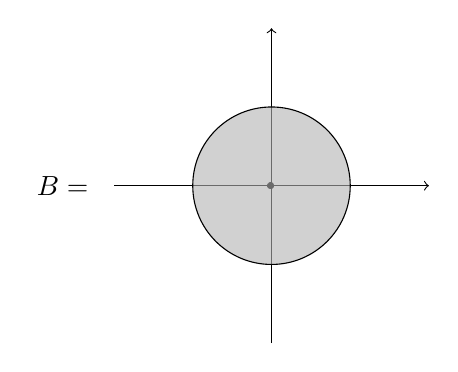
\begin{tikzpicture}[scale = 2]
                    \draw[->] (0,-1) -- (0,0) node {\tiny \textbullet} -- (0,1);
                    \draw[->] (-1,0) -- (0,0) -- (1,0);
                    \fill[black!30, opacity = 0.6] (0,0) circle (0.5);
                    \draw (0,0) circle (0.5);
                    \draw (-1.1,0) node[left] {$B=$};
            \end{tikzpicture}
        \end{center}

    \subsection{Verknüpfungen von A und B}
        \[A+B  \coloneqq  \{a + b : a \in A, b \in B\}\]
        Diese wird \mim{Dilation} genannt.
        Anschaulich wird an jeden schwarzen Punkt des Bildes $A$ das Struktur Element $B$ gelegt.
        \begin{center}
            \begin{tikzpicture}
                \draw (0,0) node[left] {$A+B=$} node[right] {\includegraphics[scale = 0.2]{Bild1dil.png}};
            \end{tikzpicture}
        \end{center}
        Bild erzeugt in Matlab durch:
        \begin{lstlisting}
I=imread('Bild1.png');
se=strel('disk',40,8);
I2=imcomplement(imdilate(imcomplement(I),se));%Es wird das Komplement des Bildes gebildet, damit das Strukturelement auf den schwarzen Bereich angewendet wird
imshow(I2);
        \end{lstlisting}

        \[A-B  \coloneqq  \{a \in A: a + B \subset A\}\]
        Diese wird \mim{Erosion} genannt.
        Anschaulich werden die schwarzen Bereiche des Bildes gesucht, in die das Strukturelement hinein passt.
        \begin{center}
            \begin{tikzpicture}
                \draw (0,0) node[left] {$A-B=$} node[right] {\includegraphics[scale = 0.2]{Bild1erode.png}};
            \end{tikzpicture}
        \end{center}

        Bild erzeugt in Matlab durch:
        \begin{lstlisting}
I=imread('Bild1.png');
se=strel('disk',20,8);
I2=imcomplement(imerode(imcomplement(I),se));
imshow(I2);
        \end{lstlisting}
        Es ist schnell zu erkennen, dass $A \neq (A+B)-B$ gilt, deshalb wird eine neue Operation eingeführt:
        \[A \bullet B  \coloneqq  (A+B)-B\]
        Dieses wird \mim{Schließen} genannt und wird etwa genutzt um Löcher, z.b. Rauschen, in einem Bild zu entfernen. Im Beispiel Bild ist zu sehen, dass das obere Fenster nicht mehr vorhanden ist.
        \begin{center}
            \begin{tikzpicture}
                \draw (0,0) node[left] {$A \bullet B=$} node[right] {\includegraphics[scale = 0.2]{Bild1close.png}};
            \end{tikzpicture}
        \end{center}
        Bild erzeugt in Matlab durch:
        \begin{lstlisting}
I=imread('Bild1.png');
se=strel('disk',20,8);
I2=imcomplement(imdilate(imcomplement(I),se));
I3=imcomplement(imerode(imcomplement(I2),se));
imshow(I3);
        \end{lstlisting}

        Es existiert auch die Umgekehrt Operation:
        \[ A \circ B  \coloneqq  (A-B)+B\]
        Diese wird \mim{Öffnen} genannt.

        Diesmal mit einem neuen Beispiel:
        \begin{center}
            \begin{tikzpicture}
                \draw (0,0) node[left] {$A=$} node[right] {\includegraphics[scale = 0.2]{Bild2.png}};
            \end{tikzpicture}
        \end{center}

        \begin{center}
            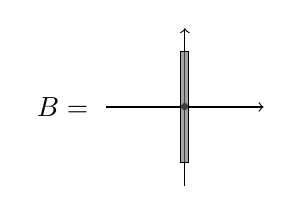
\begin{tikzpicture}
                \draw[->] (0,-1) -- (0,0) node {\tiny \textbullet} -- (0,1);
                \draw[->] (-1,0) -- (0,0) -- (1,0);
                \fill[black!60, opacity = 0.6] (-0.05,-0.7) rectangle (0.05,0.7);
                \draw (-0.05,-0.7) rectangle (0.05,0.7);
                \draw (-1.1,0) node[left] {$B=$};
            \end{tikzpicture}
        \end{center}

        \begin{center}
            \begin{tikzpicture}
                \draw (0,0) node[left] {$A \circ B =$} node[right] {\includegraphics[scale = 0.2]{Bild2open.png}};
            \end{tikzpicture}
        \end{center}

        Bild erzeugt in Matlab durch:\\
        \begin{lstlisting}
I=imread('Bild2.png');
se=strel('line',10,90);
I2=imcomplement(imerode(imcomplement(I),se));
I3=imcomplement(imerode(imcomplement(I2),se));
imshow(I3);
        \end{lstlisting}
